% Final manuscript, version 3 (merged): structure and layout of the first author's draft v2, with every
% statement of method and result taken from the verified version (docs/manuscript/ieee/main.tex) and
% checked against the code and the sealed packages. See README_FINAL_V3_EN.md in this folder.
\documentclass[5p,twocolumn]{elsarticle}

\usepackage[utf8]{inputenc}
\usepackage[T1]{fontenc}
\usepackage{amsmath,amssymb}
\usepackage{graphicx}
\usepackage{booktabs}
\usepackage{multirow}
\usepackage{array}
\usepackage{adjustbox}
\usepackage{url}
\usepackage{xcolor}
\usepackage[hidelinks]{hyperref}

% Content that is already written but must be confirmed or completed by the authors carries a
% visible marker. REMOVE EVERY \pending{...} BEFORE SENDING (grep -n "pending{" main.tex).
\newcommand{\pending}[1]{\textcolor{red}{\textbf{[PENDING: #1]}}}

\graphicspath{{../figures/}}
\biboptions{sort&compress}
\journal{Simulation Modelling Practice and Theory}

\begin{document}

\begin{frontmatter}

\title{When Proximity Is Not Interception: Auditing Capture Endpoints and Predictive Lane Blocking for Vehicle Pursuit in Microscopic Urban Traffic Simulation}

\author[1]{Andrei Noguera Gil\corref{cor1}\fnref{orcid1}}
\ead{0187940@up.edu.mx}
\author[1]{Felix Martinez-Rios\fnref{orcid2}}
\ead{fmartin@up.edu.mx}
\author[2]{Edgar Avalos-Gauna\fnref{orcid3}}
\ead{ea37@rice.edu}
\cortext[cor1]{Corresponding author.}
\fntext[orcid1]{ORCID: 0009-0007-4585-2177}
\fntext[orcid2]{ORCID: 0000-0002-2346-5922}
\fntext[orcid3]{ORCID: 0000-0002-3774-8966}

\affiliation[1]{organization={Universidad Panamericana, Facultad de Ingenier\'{\i}a},
            addressline={Augusto Rodin 498},
            city={Ciudad de M\'exico},
            postcode={03920},
            country={M\'exico}}

\affiliation[2]{organization={Rice University},
            addressline={6100 Main Street},
            city={Houston},
            state={Texas},
            postcode={77005-1827},
            country={United States}}

\begin{abstract}
Multi-vehicle pursuit is commonly scored by proximity, for example a pursuer within 5\,m of the evader. We audit what
such endpoints measure in microscopic urban traffic, using SUMO on fifteen real downtown networks. Our
endpoint, operational capture, requires a pursuer directly ahead of a nearly stopped evader, 0.3--2\,m apart, for
2\,s. First, a team that does not pursue scores 2--3\% on operational capture but 21--42\% on proximity endpoints,
and on two held-out sets of four cities a 5\,m rule reports three to five times more successes. In the official
environments of two published methods, none of 3\,379 captures joined vehicles in the same lane, and a randomly
turning team met the success criterion in 31--59\% of episodes, against 2--11\% for a chasing team. The 12-point
advantage of one controller over another vanishes under the 5\,m body-gap rule and reverses under the
centre-distance rule. Operational capture persisted in all 1\,433 audited captures with pursuers held, but an active
lane-change probe released 15. Second, a junction-level containment indicator lets 72--82\% of certified evaders
escape, against about 8\% for a lane-level indicator. Third, under operational capture, predictive lane blocking
(pursuers wait in the evader's predicted exit lanes) outperforms pursuit on both held-out sets, by 14.5 points
(97.5\% interval 8.6--20.7) and by 6.4 points (1.5--11.4); removing joint assignment costs 7.1 points. It
holds against an evader tuned against that controller, under two alternative kinematic models and with
background traffic. We propose a reporting checklist.
\end{abstract}

\begin{highlights}
\item A team that does not pursue scores 21--42\% success under proximity endpoints
\item A 5 m rule reports three to five times more captures than an operational stop
\item In two published environments no capture joined vehicles in the same lane
\item Predictive lane blocking beats pursuit on two held-out sets of real cities
\item A six-item checklist for reporting capture endpoints in pursuit studies
\end{highlights}

\begin{keyword}
multi-vehicle pursuit \sep police interception \sep evaluation methodology \sep microscopic traffic simulation \sep SUMO \sep multi-agent reinforcement learning
\end{keyword}

\end{frontmatter}

% =====================================================================================================
\section{Introduction}
\label{sec:introduction}

Intercepting a fleeing vehicle has an operational end: the fugitive car must be brought to a stop and held. Research
on multi-agent pursuit has moved from differential games \cite{isaacs1965,chung2011} and games on graphs
\cite{aigner1984,parsons1978,fomin2010,crytser2020} to multi-agent reinforcement learning (MARL) in urban traffic
simulators \cite{yuan2022t3omvp,li2024pepcrl,yang2022gradedq,li2023dgmarl,wang2022opponent}. Police interception has
also been studied as simulation--optimization on road networks
\cite{vandroffelaar2024simopt,vandroffelaar2025graph,vandroffelaar2025behavior}.

Success in learning-based pursuit is commonly scored by proximity: a shared cell or node, or a pursuer within a fixed
radius, which is 5\,m in SUMO-based studies \cite{li2024pepcrl,li2023dgmarl}. Proximity is a reasonable proxy on small
grids. In real downtowns, however, multi-lane roads and opposing traffic bring cars close to each other without
stopping anyone. For a simulation study this is a question of validity: does the event that the simulator scores
stand for the operational outcome of interest?

We audit what proximity endpoints measure in microscopic urban traffic, in the SUMO simulator \cite{lopez2018sumo} on
fifteen real downtown networks. The reference is an endpoint that we call \emph{operational capture} (OC): a pursuer
directly ahead of a nearly stopped evader, with a gap of 0.3--2\,m between the two bodies, held for 2\,s
(Section~\ref{sec:endpoints}). The audit yields three findings:
\begin{enumerate}
\item \textbf{Proximity is not interception.} A team that does not pursue scores 2--3\% on OC but 21--42\% on
proximity endpoints, and on two held-out sets of four cities a 5\,m rule reports three to five times more successes
than OC for a team that pursues. In the official environments of two published methods
\cite{li2023dgmarl,li2024pepcrl}, none of 3\,379 capture events joined two vehicles in the same lane, and a team that
turns at random met the published success criterion several times as often as a team that chases. The endpoint also
changes which controller looks better: a 12-point advantage under OC vanishes under one proximity rule and reverses
under the other. OC itself was audited: it persisted in all 1\,433 audited captures with the pursuers held, but an
active lane-change probe released 15.
\item \textbf{Containment indicators need auditing.} A junction-level indicator lets 72--82\% of the evaders that it
certifies as enclosed escape. A lane-level indicator lets about one in twelve escape, so it is useful but fallible.
\item \textbf{Waiting ahead beats chasing, and assignment matters.} Under OC, predictive lane blocking (PLB), in which
pursuers wait in the evader's predicted exit lanes, outperforms pursuit in single-shot evaluations on two held-out
sets of cities, by 14.5 points (97.5\% interval [8.6, 20.7]) and by 6.4 points ([1.5, 11.4]), and against five evader
behaviours, one of them tuned against PLB itself. A same-budget ablation shows that the joint assignment of blocking
lanes adds 7.1 points of capture.
\end{enumerate}

\emph{What is not new.} We do not claim that getting ahead of an evader is new. Prepositioning at chokepoints is
established in fugitive interception \cite{vandroffelaar2024simopt,vandroffelaar2025graph}, and anticipatory capture in
continuous spaces \cite{chen2026ambush}. Nor is stopping the target new as the objective of a learned interceptor:
agents have been trained to reach a target vehicle and then stop it in a simulated multi-lane traffic flow
\cite{bykov2025interceptor}. What we add is an audit of what capture endpoints measure, and an evaluation of
controllers under the audited endpoint.

We also report what did not help for the controllers and budgets tested (an oracle evader model, faster pursuers and
Kolmogorov--Arnold models) and a learning study that was repeated twice, after audits found defects in its training
code. We probe three limits of the study (the simulator's kinematic model, background traffic and the scripted
evader), and we close with a six-item reporting checklist. Audit details, full tables and secondary analyses are in
the supplementary material.

% =====================================================================================================
\section{Related Work and Simulation Benchmark Landscape}
\label{sec:related}

Table~\ref{tab:settings} contrasts the settings behind reported pursuit success with the setting of this work.

\begin{table*}[!t]
\centering
\caption{Settings behind reported pursuit success, and the setting of this work.}
\label{tab:settings}
\small
\setlength{\tabcolsep}{4pt}
\begin{adjustbox}{max width=\textwidth}
\begin{tabular}{@{}lllll@{}}
\toprule
Work & World & Teams & Evader & Capture \\
\midrule
T3OMVP \cite{yuan2022t3omvp} & grid, $13^2$--$21^2$ cells & 2--8 vs 4 & scripted & same cell \\
PEPCRL-MVP \cite{li2024pepcrl} & SUMO grids and a real map & 6--8 vs 3--5 & random routes & within 5\,m \\
DGMARL-MVP \cite{li2023dgmarl} & SUMO grid, 16 junctions & 4--7 vs 2--4 & random turns & within 5\,m, evader removed \\
Opponent-aware \cite{wang2022opponent} & SUMO, team-to-team & teams & pre-trained policies & pursuit time \\
Grasper \cite{li2024grasper} & graphs, 100--372 nodes & 5 vs 1 & blind, picks an exit & same node \\
AMBUSH \cite{chen2026ambush} & continuous, obstacles & slower pursuers & heuristic, human & capture range \\
Evader-agnostic \cite{kalanther2025evader} & grid, occlusion; AirSim & team vs 1 & fictitious, varying rationality & detect and intercept \\
Interceptor agents \cite{bykov2025interceptor} & cellular automaton, 3-lane ring & 1--2 vs 1 & non-reactive vehicle & target speed zero \\
Our earlier study \cite{noguera2025kan} & SUMO, one OpenStreetMap network & 2 vs 1 & static & within 20\,m \\
This work & SUMO, 15 real downtowns & 3--7 vs 1 & 5 scripted behaviours, one tuned & operational stop (OC) \\
\bottomrule
\end{tabular}
\end{adjustbox}
\end{table*}

\subsection{Pursuit on Graphs and Learning-Based Multi-Vehicle Pursuit}

Pursuit--evasion on graphs dates back to Parsons \cite{parsons1978}. Three cops suffice on planar graphs
\cite{aigner1984}. Against a faster robber, the number of cops required on planar graphs is unbounded
\cite{fomin2010}. Containment requires occupying every edge at the robber's vertex \cite{crytser2020}. Surveys cover
search and pursuit--evasion in robotics \cite{chung2011}, and differential games treat continuous pursuit
\cite{isaacs1965}.

In learning-based multi-vehicle pursuit, SUMO-based studies use grids and, in PEPCRL-MVP, a real map, with proximity
capture \cite{li2024pepcrl,li2023dgmarl,yang2022gradedq}. In DGMARL-MVP the evader is removed from the simulation at
capture, so what happens after the encounter cannot be observed. Opponent-aware team-to-team pursuit uses pre-trained
evader policies \cite{wang2022opponent}. Generalist graph pursuers capture on a shared node
\cite{li2024grasper,lu2025equilibrium}, and decentralized deep-RL pursuit has also been studied for kinematic agents
\cite{desouza2021}. Evader-agnostic team pursuit under occlusion trains against fictitious evaders of varying
rationality \cite{kalanther2025evader}. Concurrently, Chen et al.\ \cite{chen2026ambush} study ambush strategies for
slower pursuers in obstacle-rich continuous spaces. In an earlier study we trained two decentralized pursuers by
multi-agent reinforcement learning against a static prey on one SUMO network, and interpreted the learned policies
with a Kolmogorov--Arnold network \cite{noguera2025kan}. That study named a static prey and a team of two
as its limits, and left larger teams and more complex urban environments to future work. Its capture rule, which that article does not state, was a distance below 20\,m between a
pursuer and the prey in the code that survives, and it was not audited: it is an instance of the proximity scoring
examined here.

\subsection{Learning to Stop a Vehicle}

Closest to our objective, Bykov et al.\ \cite{bykov2025interceptor} train one or two interceptor agents by
reinforcement learning on a three-lane ring road modelled as a stochastic cellular automaton. The target is an
ordinary vehicle of the flow and does not react to the interceptors. An interceptor first reaches the target, to
within six cells, where it is compared with four heuristic drivers, and then slows it by driving in front of it.
Stopping is measured by the time until the target first has zero speed and by the share of time steps in which it is
stopped. One agent slows the target but generally does not stop it; two agents that block two of the three lanes do.
Stopping instead of approaching is therefore not our contribution, and neither is a learned controller that stops a
vehicle. Our study differs in two ways. Its setting has what those authors list as limits of theirs: a road network
with junctions instead of a ring, and evaders that react to the pursuers. And it examines the endpoint itself: we
contrast an operational stop with proximity on the same episodes, measure both with a team that does not pursue,
follow each capture for 60\,s, audit the capture events of published environments, and evaluate at lane level on
real road networks.

\subsection{Simulation--Optimization and Network Interdiction}

Simulation--optimization positions police units at chokepoints of a fugitive's possible routes in real time
\cite{vandroffelaar2024simopt}. Related work studies graph coarsening \cite{vandroffelaar2025graph} and sensitivity
to models of fugitive behaviour \cite{vandroffelaar2025behavior}. Closest to our setting, vehicle interdiction has
been optimized and assessed in SUMO on a real campus network, with a fugitive that chooses routes
\cite{samanta2021interdiction,samanta2024interdiction}. That work covers both static allocation of police resources
and routes and schedules of defender vehicles that tour the network and wait, so moving defenders are not new. Its
success criterion is a defender within a distance threshold of the fugitive (30\,m in the preprint), which is a
proximity endpoint. Our study differs in what it measures: an audited operational stop contrasted with proximity on
the same episodes, lane-level blocking, closed-loop re-planning against reactive evaders, and evaluation on held-out
cities. Network interdiction removes arcs to lengthen an adversary's shortest path \cite{wood1993,israeli2002}. PLB
shares the idea of getting ahead and blocking, so its value here is that of a baseline evaluated under an audited
microscopic endpoint. It is not a new principle.

\subsection{Simulation Credibility and Evaluation Practice}

A simulation model is valid only with respect to the purpose for which it is used \cite{sargent2013}. For a
pursuit benchmark, that purpose includes the event that is scored as success: the conclusions are credible only to
the extent that this event represents the outcome that the study is about. Statistical practice in deep RL \cite{agarwal2021,henderson2018} and the gap between proxies and goals
\cite{skalse2022} motivate our approach: pre-registered paired comparisons with clustered bootstrap intervals
\cite{efron1993}, audits of proxies against the outcomes they stand for, and a single-shot hold-out evaluation.
Caging and herding of moving agents give explicitly scoped containment guarantees \cite{varava2017}; our containment
indicators are operational and are evaluated empirically.

On the learning side, PPO \cite{schulman2017ppo} and MAPPO \cite{yu2022mappo,lowe2017maddpg} are standard for
cooperative tasks. Kolmogorov--Arnold networks \cite{liu2025kan} replace fixed activations by learnable splines.
Accumulated local effects \cite{apley2020ale} address the bias of partial dependence under correlated predictors.

% =====================================================================================================
\section{Simulation Environment}
\label{sec:setting}

\subsection{Simulator and Microscopic Model}

We use SUMO 1.21 through TraCI \cite{lopez2018sumo}, with 0.1\,s physical steps, 1\,s decisions and a 300\,s horizon.
Car-following is the Krau{\ss} model \cite{krauss1998} with $\sigma=0.5$, and lane changing uses SUMO's model
\cite{erdmann2015}. Teleporting is disabled. Bodies are $5.0\times1.8$\,m. The minimum gap is 2.5\,m for pursuers and
1.0\,m for the evader. A collision is a physical overlap of bodies, and safety checks stay on. Our experiments do not
include reversing or mid-edge U-turns.

\subsection{Road Networks}

We use fifteen downtown networks built from OpenStreetMap. Eleven were split before any experiment:
\begin{itemize}
\item TRAINING: Adelaide, Toronto, Washington, Seattle;
\item DEVELOPMENT: Phoenix, Portland, Sapporo;
\item TEST: Chicago, Melbourne, Salt Lake City, Minneapolis.
\end{itemize}
The parameter searches of PLB and of the tuned evader used the TRAINING cities only. DEVELOPMENT cities were not used by the parameter search, but they
informed design decisions; we call the seven together the development-phase cities. TEST was opened once, for a
single-shot evaluation with frozen methods (Section~\ref{sec:test}). A second held-out set, HELD-OUT~B (Denver,
Vancouver, Barcelona, Buenos Aires), was added after every method and analysis had been frozen. Its cities and their
acceptance criteria were registered before any map was downloaded, the networks were built with the recipe of the
existing ones, and the set was evaluated once. Two controlled grids represent the regime of the literature.

\subsection{Evader Behaviour Models}

The evader is scripted and deterministic given its seed, and it decides its next edge shortly before each junction
from the pursuers' current positions:
\begin{enumerate}
\item \emph{Random} chooses uniformly among the continuations.
\item \emph{Avoidant} maximizes the graph distance to the nearest pursuer over a random pair of continuations.
\item \emph{Optimal} maximizes that distance over all continuations.
\item \emph{Goal-directed} drives to a far destination at the edge of downtown, avoiding continuations that end
within 150\,m of a pursuer.
\item \emph{Tuned} scores each continuation by a weighted sum of seven features of the pursuers' current positions,
with weights searched to minimize capture by PLB. It is used in one study (Section~\ref{sec:evaders}).
\end{enumerate}

\subsection{Pursuers and Scenarios}

Teams have 3, 5 or 7 pursuers with the evader's speed. A command is ``drive to edge $e$ and stop $h$\,m into lane
$\ell$''. It is admitted only if it can be followed at ordinary deceleration (4.5\,m/s$^2$).

A frozen generator places the evader on an edge with at least two continuations, and the pursuers at 100--800\,m
route distance from it. Placements are nested across team sizes. Every contrast is paired by scenario and SUMO seed.
A \emph{family} is a city, a scenario and an evader behaviour; the team-size cells of a family share starts.

% =====================================================================================================
\section{Endpoints and Indicators}
\label{sec:endpoints}

\begin{figure*}[!t]
\centering
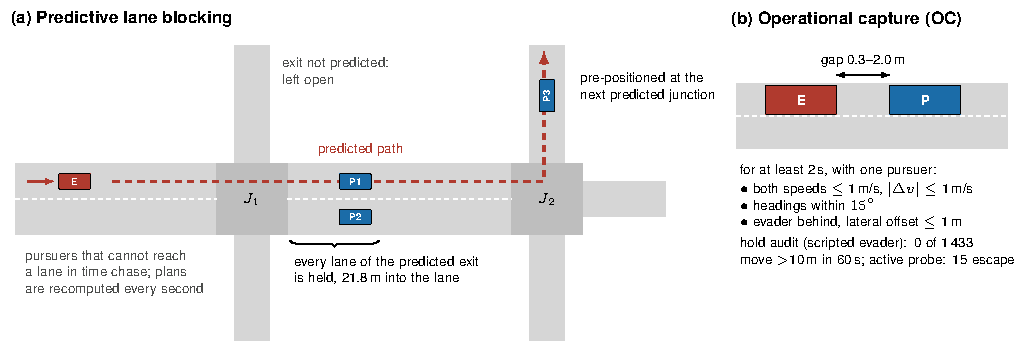
\includegraphics[width=\textwidth]{F0_method.pdf}
\caption{(a) Predictive lane blocking. The evader's path is predicted greedily: at each junction, the continuation that
maximizes its time lead over the nearest pursuer. Pursuers drive ahead and stop in the lanes of the predicted exits,
when they can reach them in time; otherwise they chase. Plans are recomputed every second. (b) The operational capture
(OC) endpoint. The schematic was drawn as vector code with the assistance of Claude Opus~5.5 (Anthropic) from the
authors' description of the method, and was reviewed by the authors for accuracy.}
\label{fig:method}
\end{figure*}

\subsection{The Operational Capture Predicate}

Let $c_i(t)\in\mathbb{R}^2$, $\theta_i(t)$ and $v_i(t)$ be the centre, the heading and the speed of pursuer
$i\in\{1,\dots,N\}$ at time $t$, and $c_e(t)$, $\theta_e(t)$ and $v_e(t)$ those of the evader. Let $g_i(t)$ be the
\emph{body gap}, the smallest distance between the rectangular bodies of pursuer $i$ and of the evader. With
$d_i=c_i-c_e$, $u_i=(\cos\theta_i,\sin\theta_i)$ and $n_i=(-\sin\theta_i,\cos\theta_i)$, the contact condition of
pursuer $i$ at time $t$ is
\begin{align}
\label{eq:contact}
\kappa_i(t) \iff{} & 0.3 \le g_i \le 2.0\ \text{m} \nonumber \\
& \wedge\ \max(v_i,v_e) \le 1\ \text{m/s} \ \wedge\ |v_i-v_e| \le 1\ \text{m/s} \nonumber \\
& \wedge\ |\theta_i-\theta_e| \le 15^\circ \nonumber \\
& \wedge\ d_i\cdot u_i > 0 \ \wedge\ |d_i\cdot n_i| \le 1\ \text{m},
\end{align}
where the difference of headings is taken on the circle. The bound on the relative speed belongs to the registered
predicate; it is implied by the two bounds on the speeds. The four lines require, in turn, a close gap without
contact, a near stop of both vehicles, aligned headings, and the evader behind the pursuer and in file with it.
Operational capture holds at time $t$ when one pursuer satisfies the contact condition throughout a dwell of
$T=2$\,s:
\begin{equation}
\label{eq:oc}
\mathrm{OC}(t) \iff \exists\, i\ \ \forall\, \tau\in[t-T,\,t]:\ \kappa_i(\tau),
\end{equation}
evaluated at every physical step (Fig.~\ref{fig:method}b). The capture time is the earliest such $t$. The order of
the quantifiers matters: the dwell must be held by one and the same pursuer, so a sequence of brief contacts with
different pursuers does not count. The predicate has no condition on lane identity. The lateral bound excludes two
vehicles stopped side by side in adjacent lanes.

The pursuers' 2.5\,m gap keeps a trailing pursuer outside the band. The evader's 1.0\,m gap, however, places it inside
the band whenever it stops or crawls behind a pursuer, including during ordinary slow following. OC therefore measures
operational close stopping behind a pursuer. It does not prove that escape is physically impossible, and it requires
no rear blocker. We quantify its incidental matches with a null team, and its persistence with a hold audit.

\subsection{Proximity Endpoints}

The proximity endpoints, which we use for calibration only, hold when some pursuer is close to the evader at any
instant of the episode:
\begin{align}
\label{eq:prox}
\phi^{\mathrm{gap}}_{d} &\iff \exists\, i,\ t:\ g_i(t) \le d, \qquad d\in\{5\ \text{m},\,10\ \text{m}\}, \nonumber \\
\phi^{\mathrm{ctr}} &\iff \exists\, i,\ t:\ \lVert c_i(t)-c_e(t)\rVert \le 5\ \text{m}.
\end{align}
We call the first the body-gap rule and the second the centre-distance rule. Neither constrains speed, heading or
duration.

\subsection{Persistence Audit}

Each captured episode is re-simulated with every pursuer held at speed 0 from the capture on. The horizon is extended
where necessary, so that every capture has 60\,s of follow-up. The evader escapes if it moves more than 10\,m within
60\,s. This tests persistence against the scripted evaders and SUMO's lane changing, not against every admissible
manoeuvre.

\subsection{Containment Indicators}

A free-flow search from the evader defines \emph{safe} junctions, which the evader reaches 0.5\,s before every
pursuer, and \emph{gates} on their frontier. An indicator fires when there are at most two safe junctions and every
gate is held for 10\,s:
\begin{itemize}
\item \emph{junction-level}: a pursuer is within 25\,m of the gate at no more than 2\,m/s;
\item \emph{lane-level}: every lane by which the evader would enter the gate carries a stopped pursuer ahead of the
evader, and at least one gate exists.
\end{itemize}
Fired indicators are re-simulated, with all pursuers keeping their last command. \emph{Joint escape} is defined as
entering an edge that leaves a gate, or leaving the network, within a complete 60\,s follow-up.

% =====================================================================================================
\section{Interception Strategies}
\label{sec:strategies}

\subsection{Pursuit and Junction Ambush}

\emph{Pursuit.} Every pursuer drives to the end of the evader's current edge.

\emph{Junction ambush.} The planner predicts the evader's path greedily (Fig.~\ref{fig:method}a): at each junction it
takes the continuation that maximizes the evader's time lead over the nearest pursuer. For a junction $J$ on that
path, let $\mathcal{L}(J)$ be the set of all lanes of all the exits that the evader can take there, $t_e(J)$ the predicted
arrival time of the evader, and $c(i,\ell)$ a conservative estimate of the time that pursuer $i$ needs to reach its stopping point in lane
$\ell$. The team can close $J$ when it has at least as many pursuers as $J$ has exit lanes and the best one-to-one
assignment $\pi$ of pursuers to lanes leaves enough slack:
\begin{equation}
\label{eq:assign}
\max_{\pi}\ \min_{\ell\in\mathcal{L}(J)}\ \bigl[\,t_e(J)-c(\pi(\ell),\ell)\,\bigr] \ \ge\ m .
\end{equation}
The planner takes the nearest such junction and sends the assigned pursuers to stop in their lanes; the other
pursuers chase. The slack $m$ is 2\,s. The maximum is found by enumeration.

\subsection{Predictive Lane Blocking (PLB)}

PLB adds pre-positioning: when a full ambush is infeasible, pursuers wait in the predicted exit lanes of the next one
or two junctions. The pursuers decide in a fixed order; each takes the best lane that it can reach in time, with the
evader's predicted exit first and the nearer junction next, and it excludes the lanes already taken by teammates.
Pursuers that can reach no such lane in time chase. Plans are recomputed every second. The team ambush of
Eq.~\eqref{eq:assign} is kept; for teams larger than five, PLB replaces the enumeration by a greedy rule that serves
the hardest lane first. PLB's eight timing parameters, the slack $m$ among them, were optimized on TRAINING cities by
random search with successive halving \cite{bergstra2012,jamieson2016,li2018hyperband}, with a breaker requiring a
gain of 0.02 over the defaults.

\subsection{Counterfactual Controllers}

\emph{Singles} run PLB with one pursuer alone from its team start. \emph{Oracle PLB} uses a copy of the evader's
decision function. \emph{Independent PLB} (coordination ablation) keeps PLB's prediction, information and per-pursuer
rule, but removes joint assignment: there is no team ambush, and each pursuer chooses its waiting lane as if alone,
without excluding lanes chosen by teammates.

\subsection{Learned Controllers}

A centralized-critic PPO in the style of MAPPO, with a shared actor (MLP or KAN head), lets each pursuer choose a
blocking lane, chase or stay every 3\,s. The actor is sequential: pursuers decide in a fixed order, and each sees the
choices made earlier in the same step. The controller is behaviour-cloned from PLB and then fine-tuned with circuit
breakers, on all city--setting combinations, with OC as the reward and the selection rule. It is our own adaptation,
not a published method run as released. Fine-tuning was run with three implementations. In the first (MAPPO-v2), an
audit found that the critic received a state built after the actions it was meant to judge, and that sampling was not
controlled by the declared seed. The second (MAPPO-v3) corrects both. A later audit found two further defects in the
training loop of both; the third (MAPPO-v4) corrects them (Section~\ref{sec:limit}). Every learning result is
labelled by its implementation. An option-PPO study and a further controller (cut) are described in the supplement
(Sections~S-III and S-IV).

% =====================================================================================================
\section{Experimental Protocol and Statistics}
\label{sec:protocol}

Confirmatory studies were pre-registered: protocol, primary hypothesis and analysis were recorded, and sources hashed,
before launch. Analyses marked \emph{post hoc} were not pre-registered. Registration is internal, through sealed
packages with SHA-256 checksums; it is not externally timestamped. Original outputs are never relabelled. Later
corrections (follow-up completion, joint escape, clustered intervals) are versioned addenda, listed in the supplement
(Section~S-VIII) together with the count of episodes behind every result.

\emph{Uncertainty.} Rates are averaged over SUMO seeds within each scenario cell, and differences are paired.
Intervals are percentile bootstraps (10\,000 resamples) over families, so that all team-size cells of a family move
together. We also report two-stage city~$\to$~family intervals; with four cities in each held-out set,
population-level inference about cities remains limited. Intervals are given in square brackets after the estimate,
with their level.

\emph{Independence reference.} We compare team capture with $1-\prod_i(1-p_i)$, where $p_i$ is the capture rate of
pursuer $i$ alone from the same start, estimated from two SUMO replicates. This is a reference under an independence
model, not a causal decomposition. The evader meets different situations in solo and team worlds, so a non-positive
excess does not prove that coordination is absent.

\emph{Use of AI tools in the research.} Two AI models were used in the research process and not only in writing,
at several reasoning-effort settings and under the supervision of the first author. Claude Opus~5.5 (Anthropic),
through Claude Code in the Claude desktop application, was used for creation: it wrote and edited the simulation,
controller, training and analysis code, ran the experiments, computed the statistics, and produced the data figures
with a script, directly from the sealed result files; no figure showing results was generated or altered by an image
model. Astra, through the ChatGPT desktop application (OpenAI), was used for verification: it helped the first author
and his advisor to check the progress, the code and the quality of the work in six rounds of audit. The first author
decided the questions, the designs, the hypotheses registered before each run, and whether a study was repeated or
stopped; these decisions are recorded with their dates. The safeguards against errors in AI-written code were more
than 500 unit tests, among them tests that reproduce each defect found; sealed result packages with checksums; a
script that checks every number of the text against the sealed summaries; and the six rounds of audit, which found
defects in the training code that were corrected and are reported (Section~\ref{sec:limit}). The same standards of
validity and reproducibility apply to this code as to any other, and it is released with the data.

% =====================================================================================================
\section{Finding 1: Proximity Is Not Interception}
\label{sec:measurement}

\subsection{A Team That Does Not Pursue}

\begin{figure}[!t]
\centering
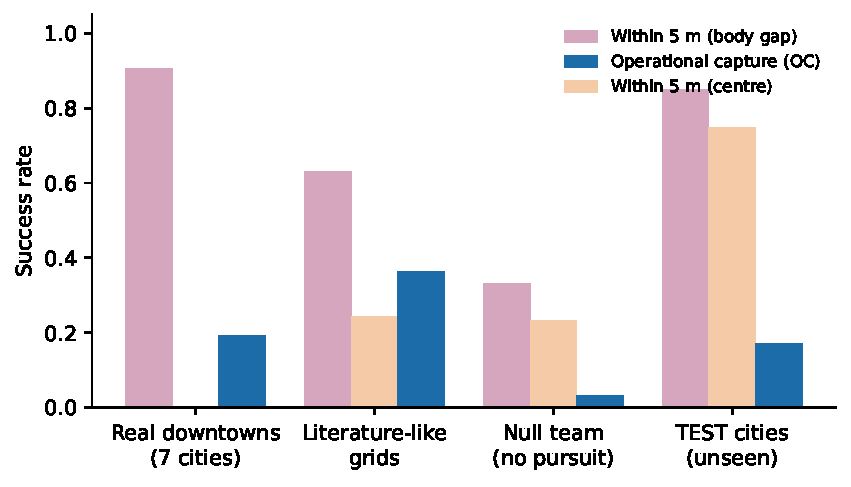
\includegraphics[width=\columnwidth]{F1_endpoint_calibration.pdf}
\caption{Success under proximity endpoints and under operational capture (OC). The null team does not pursue. Real
downtowns and TEST cities: pursuit team.}
\label{fig:endpoints}
\end{figure}

A null team of five pursuers that drive random routes, without pursuing, scores 3.1\% [1.5, 5.1] on OC (family 95\%
interval, 274 families). The same team scores 33.2\% [28.5, 38.1] within 5\,m (body gap), 23.4\% [19.2, 27.7] within
5\,m (centre distance) and 42.3\% [37.4, 47.5] within 10\,m (Fig.~\ref{fig:endpoints}; 548 episodes on seven cities).
On the four cities of HELD-OUT~B the same team scores 1.6\% on OC, 27.3\% within 5\,m (body gap) and 21.4\% within
5\,m (centre distance). Proximity endpoints thus register success in a large share of episodes without any pursuit,
whereas OC has a small floor of incidental matches.

\subsection{The Same Episodes Under Both Endpoints}

For the pursuit team on the four TEST cities, the pre-registered contrast body-gap 5\,m minus OC is $+0.679$ (97.5\%
family interval [0.620, 0.735]): 0.851 versus 0.172, a ratio of 4.9. With centre distance the ratio is 4.4 (0.748). On
HELD-OUT~B the same pre-registered contrast is $+0.549$ (97.5\% family interval [0.476, 0.620]): 0.776 versus 0.227,
a ratio of 3.4. On the seven development-phase cities, body-gap 5\,m success is 0.85--0.96 against an OC rate of
0.10--0.35. On small literature-like grids, the centre-distance rule is close to, or stricter than, OC (0.24 versus
0.36 for pursuit). The disagreement is therefore regime-dependent. It does not show that published results obtained
with other policies and environments are inflated; it shows that proximity and operational interception answer
different questions in real downtown traffic.

\subsection{What a Published Capture Rule Measures}
\label{sec:published}

To check that these proximity rules are not a straw man, we ran the official code of a published SUMO pursuit method,
DGMARL-MVP \cite{li2023dgmarl}, without modifying it, and observed its capture events (supplement, Section~S-II). In
the released environment, a capture is a distance below 5\,m between the front-bumper points of a pursuer and an
evader; the evader is then removed from the simulation. Vehicles are 5\,m long and every road has one lane per
direction, so a pursuer that follows the evader in its lane cannot satisfy the rule. We ran 300 episodes of the
released scenario with four pursuers and two evaders for each of two teams that use the published action space, a
turn at each junction: a \emph{null} team that turns at random, and a \emph{chaser} team in which each pursuer takes
the turn that is shortest by road to its evader (Table~\ref{tab:published}).

\begin{table}[!t]
\centering
\caption{Capture events in the official DGMARL-MVP environment (released scenario, four pursuers and two evaders,
300 episodes per team). Episode-level 95\% bootstrap intervals.}
\label{tab:published}
\small
\setlength{\tabcolsep}{4pt}
\begin{adjustbox}{max width=\columnwidth}
\begin{tabular}{@{}lcc@{}}
\toprule
& Null team & Chaser team \\
\midrule
Published success & 42.7\% [37.3, 48.3] & 4.0\% [2.0, 6.3] \\
Capture events & 398 & 139 \\
\quad same lane & 0 & 0 \\
\quad opposite directions & 82.9\% & 59.7\% \\
\quad inside a junction & 17.1\% & 40.3\% \\
\quad evader faster than 1\,m/s & 75.6\% & 90.6\% \\
\midrule
\multicolumn{3}{@{}l}{\emph{First capture, evader not removed, 10\,s later}} \\
\quad over 50\,m from every pursuer & 94.8\% [92.2, 97.4] & 92.9\% [88.2, 96.9] \\
\quad median distance to its captor & 119\,m & 102\,m \\
\bottomrule
\end{tabular}
\end{adjustbox}
\end{table}

Three observations follow. First, none of the 537 capture events (999 over both released scenarios) joined two
vehicles in the same lane: they were vehicles passing in opposite directions or crossing inside a junction, and in
most of them the evader was moving. Second, the team that turns at random met the published success criterion (all
evaders captured within 800 steps) in 42.7\% of episodes, against 4.0\% for the team that chases. Chasing places the
pursuer behind the evader, where the rule cannot fire. Third, when the evader of the first capture was left in the
simulation, it was more than 50\,m from every pursuer 10\,s later in 93--95\% of cases.

For reference, the article reports success rates of 0.77--0.91 for four learned methods in this scenario
\cite{li2023dgmarl}. Those figures are not comparable with ours in detail: the released configuration differs from the
reported one, we used a later SUMO version, and we did not train the published learner. The audit therefore says
nothing about the quality of that learner. It shows what the endpoint rewards in this environment: crossing the
evader's path, not stopping it.

\emph{A second environment.} We repeated the audit, with its design and a prediction registered beforehand, on the
official code of PEPCRL-MVP \cite{li2024pepcrl}, whose release contains a real map with one lane per direction and
three scenarios. Each team and scenario was run for 150 seeds in two modes, the unmodified dynamics and a follow-up
mode; 884 and 897 of 900 episodes completed, and the others aborted inside the released code. As predicted, none of
the 2\,380 capture events of the unmodified mode joined two vehicles in the same lane: 76--83\% were vehicles passing
in opposite directions and 17--24\% crossings inside a junction. Of these events, 22 were recorded in episodes that
aborted afterwards; success rates use completed episodes only. The null team met the published criterion in 31.3\%
[24.0, 38.7], 59.1\% [51.0, 67.1] and 58.7\% [50.7, 66.7] of episodes in the three scenarios, against 2.8\%, 10.7\%
and 9.7\% for the chaser. Of 827 first captures followed without removing the evader, 2 were within 5\,m of their
captor 5\,s later. The article reports 0.56--0.68 for its method and 0.27--0.62 for eight baselines on this map; the
same caveats apply. Both environments come from one research group and share code, so this adds a real map and a
journal article, not an independent group (supplement, Section~S-II).

\subsection{The Endpoint Changes the Conclusion}
\label{sec:reversal}

\begin{table}[!t]
\centering
\caption{PLB and pursuit under each endpoint, on three independent sets of fresh scenarios (seven
development-phase cities; 273, 273 and 267 families). Differences with family-clustered 95\% intervals are in the
text.}
\label{tab:reversal}
\small
\setlength{\tabcolsep}{3pt}
\begin{tabular}{@{}llccc@{}}
\toprule
Set & & OC & Body gap $\le$5\,m & Centre $\le$5\,m \\
\midrule
\multirow{3}{*}{A} & PLB & 0.397 & 0.921 & 0.840 \\
& Pursuit & 0.274 & 0.934 & 0.861 \\
& Difference & $+0.123$ & $-0.013$ & $-0.021$ \\
\midrule
\multirow{3}{*}{B} & PLB & 0.400 & 0.920 & 0.823 \\
& Pursuit & 0.282 & 0.925 & 0.861 \\
& Difference & $+0.119$ & $-0.004$ & $-0.038$ \\
\midrule
\multirow{3}{*}{C} & PLB & 0.376 & 0.893 & 0.815 \\
& Pursuit & 0.248 & 0.897 & 0.836 \\
& Difference & $+0.128$ & $-0.004$ & $-0.021$ \\
\bottomrule
\end{tabular}
\end{table}

The choice of endpoint also changes which controller looks better (Table~\ref{tab:reversal}). On three independent
sets of fresh scenarios, PLB minus pursuit is $+0.123$ [0.088, 0.160], $+0.119$ [0.076, 0.160] and $+0.128$
[0.084, 0.170] under OC. Under the 5\,m body-gap rule it is $-0.013$ [$-$0.025, $-$0.004], $-0.004$
[$-$0.013, 0.004] and $-0.004$ [$-$0.011, 0.003], and under the centre-distance rule $-0.021$ [$-$0.040, $-$0.002],
$-0.038$ [$-$0.059, $-$0.020] and $-0.021$ [$-$0.038, $-$0.006]. A 12-point advantage in operational capture is
thus invisible under one proximity rule and reversed under the other. On HELD-OUT~B, where the advantage under OC is
6 points (Section~\ref{sec:test}), it is $+0.016$ [$-$0.002, 0.037] under the body-gap rule and $+0.004$ [$-$0.016,
0.025] under the centre-distance rule.

An earlier version of this study also reported that a learned controller trained with the 5\,m rule as its reward
lost 16 points of OC while its proximity score did not change. Audits then found defects in the training code
(Section~\ref{sec:limit}). In two repetitions with corrected code the loss did not recur. With the final
implementation, training on proximity for the same budget produced no detected change in OC ($-0.004$
[$-$0.014, 0.007]) and no detected widening of the gap between the endpoints ($+0.003$ [$-$0.008, 0.014]), so the
registered contrast was not met. The repetitions do not isolate what produced the earlier loss. We therefore make no
claim about what proximity rewards do to a learner (supplement, Section~S-IV).

\subsection{Does an Operational Capture Persist?}

With every pursuer held from the capture on, and a complete 60\,s follow-up, no escape was observed in 1\,433 audited
OC captures (562 by PLB, 480 by the junction ambush and 391 by pursuit). They come from 176 scenario--evader families
in seven cities and share families across methods, team sizes and seeds, so we report the count rather than an
independence-based bound. Zero observed escapes is not a guarantee that escape is impossible. If the controllers keep
re-planning after a capture, 8--14\% of evaders are later released, so an operational system should stop re-planning
at capture.

\emph{Active-escape probe.} We repeated the hold audit with a probe that, from the moment of capture, requests every
second a change to an adjacent lane with an onward link and a reroute through it, with safety checks on. Among the
1\,433 reproduced captures, 15 escapes were observed under this probe, from 3 of 176 families. OC therefore does not
guarantee containment against this manoeuvre. Lane-change requests were recorded in 115 episodes, which include all
15 escapes. In 1\,316 episodes only reroute requests were recorded, and no escape was observed; two episodes were
inconclusive. The probe did not take an independent inventory of lanes at capture, and it did not verify that a
requested manoeuvre was executed. The supplement (Section~S-I) gives the audit table, the completion of 188
originally censored follow-ups and the verification of each replay. After an audit found that the helper which
timed the captures could join two fragments of a run, all 1\,433 captures were replayed and each capture instant was
confirmed with a corrected extractor and with the judge.

% =====================================================================================================
\section{Finding 2: Containment Indicators Need Auditing}
\label{sec:indicators}

\begin{figure}[!t]
\centering
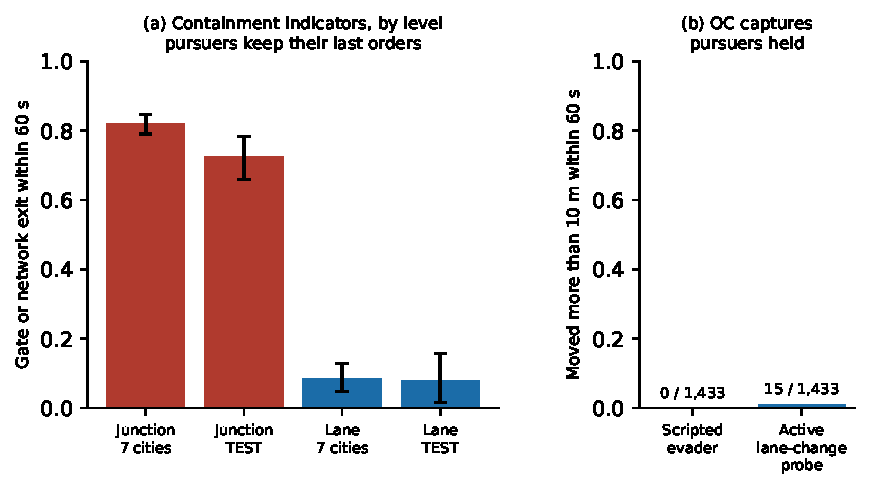
\includegraphics[width=\columnwidth]{F3_certificate_validity.pdf}
\caption{(a) Joint escape (gate or network exit) within a complete 60\,s follow-up after a containment indicator
fires, with the pursuers keeping their last orders; family-clustered 95\% intervals. (b) OC captures in which the
evader moved more than 10\,m within 60\,s with every pursuer held, for the scripted evaders and under the active
lane-change probe (counts). The two panels use different escape definitions and are not comparable bar to bar.}
\label{fig:certificates}
\end{figure}

A containment indicator certifies, during an episode, that the evader is enclosed. It could serve as a stopping rule
or as a reward only if certified evaders in fact stay enclosed, so we measured how often they escape. With complete
follow-up and joint escape (Fig.~\ref{fig:certificates}), the junction-level indicator lets 82.0\% [79.1, 84.8] (7
cities, $n=1\,098$) and 72.5\% [66.0, 78.5] (TEST, $n=848$) of evaders escape (family 95\% intervals). Its usual
failure is a pursuer parked on a different approach to the gate. The lane-level indicator lets 8.4\% [4.7, 12.9]
($n=225$, 150 families) and 7.9\% [1.7, 15.8] ($n=240$, 69 families) escape; 95--97\% of its firings coincide with an
OC capture. An earlier analysis counted gate escapes only and treated late certificates as complete. It reported
5.4--5.8\% and passed a 10\% criterion, which the joint definition does not reproduce. We therefore present the
lane-level indicator as useful but fallible.

% =====================================================================================================
\section{Finding 3: Controller Performance, Robustness and Learning}
\label{sec:results}

\subsection{Single-Shot Evaluations on Two Held-Out Sets}
\label{sec:test}

\begin{figure*}[!t]
\centering
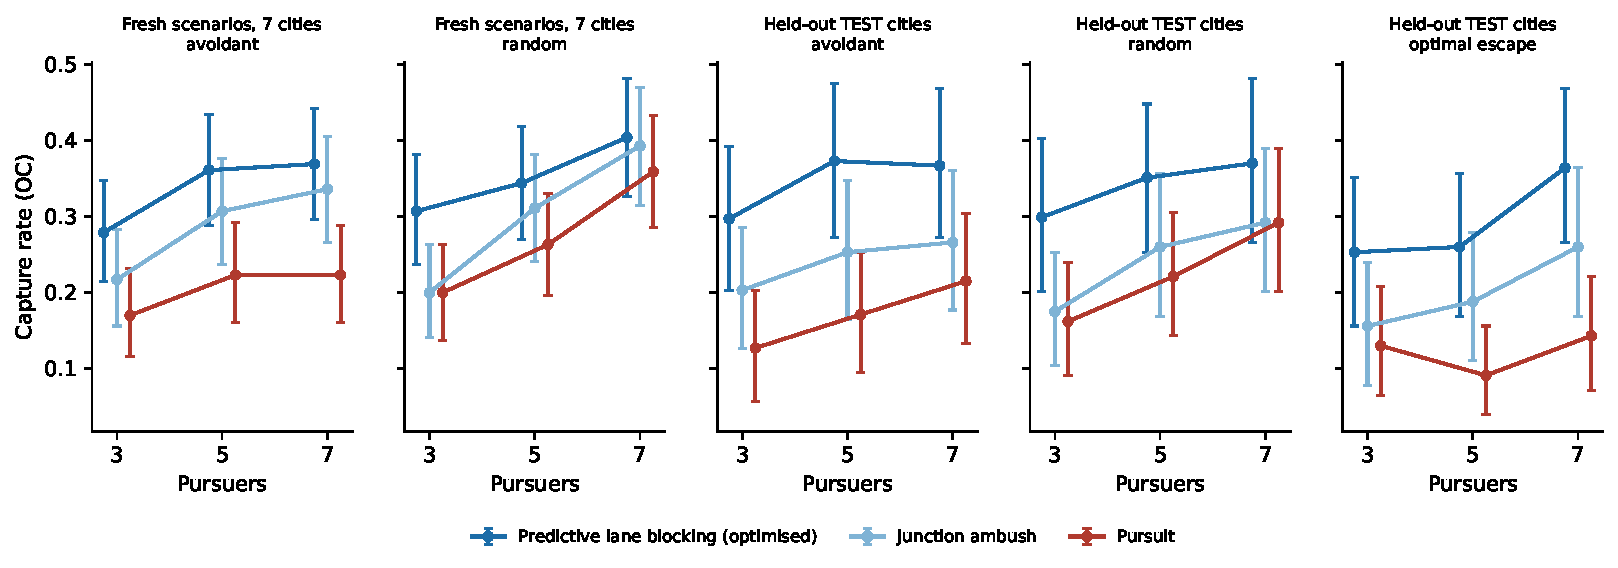
\includegraphics[width=\textwidth]{F2_methods_by_team.pdf}
\caption{Capture rate (OC) by team size. Left: fresh scenarios on seven development-phase cities. Right: single-shot
evaluation on four held-out TEST cities. Bars: 95\% bootstrap intervals over scenarios.}
\label{fig:methods}
\end{figure*}

\begin{table}[!t]
\centering
\caption{Single-shot evaluation on the four TEST cities with frozen methods. OC capture rates. 7\,200 team episodes
were scheduled for five methods; 210 failed scenario placement, identically for all methods, leaving 6\,990. The two
learned controllers of that evaluation are in the supplement (Table~S-III).}
\label{tab:test}
\small
\setlength{\tabcolsep}{5pt}
\begin{tabular}{@{}llccc@{}}
\toprule
Evader & Team & PLB & Ambush & Pursuit \\
\midrule
\multirow{3}{*}{Random} & 3 & 0.299 & 0.175 & 0.162 \\
& 5 & 0.351 & 0.260 & 0.221 \\
& 7 & 0.370 & 0.292 & 0.292 \\
\midrule
\multirow{3}{*}{Avoidant} & 3 & 0.297 & 0.203 & 0.127 \\
& 5 & 0.373 & 0.253 & 0.171 \\
& 7 & 0.367 & 0.266 & 0.215 \\
\midrule
\multirow{3}{*}{Optimal} & 3 & 0.253 & 0.156 & 0.130 \\
& 5 & 0.260 & 0.188 & 0.091 \\
& 7 & 0.364 & 0.260 & 0.143 \\
\bottomrule
\end{tabular}
\end{table}

TEST was opened once (Table~\ref{tab:test}, Fig.~\ref{fig:methods}). The pre-registered primary is PLB minus pursuit,
pooled over the avoidant and random evaders and all team sizes, on 156 families and 468 cells. It is $+0.145$. The
pre-registered bootstrap over cells gives a 97.5\% interval of [0.101, 0.189]. The corrected bootstraps, which keep
families together, give [0.086, 0.207] over families (97.5\%) and [0.074, 0.228] over cities and families (95\%). The
difference is positive in every city: Chicago $+0.11$, Melbourne $+0.06$, Minneapolis $+0.21$, Salt Lake City
$+0.20$. Against the optimal evader it is $+0.171$ (family [0.108, 0.238]), and PLB minus the junction ambush is
$+0.102$ (family [0.053, 0.151]).

HELD-OUT~B was evaluated once, with the same frozen methods and the same primary (4\,640 scheduled episodes, 4\,498
valid; 157 families and 459 cells). PLB minus pursuit is $+0.064$, with a 97.5\% family interval of [0.015, 0.114]
and a 95\% interval over cities and families of [0.009, 0.132]. The primary is met, and the advantage is less than
half of that on TEST: the difference between the two sets is $+0.081$ [0.011, 0.149] (post hoc). By city it is
$+0.15$ in Denver, $+0.03$ in Vancouver, $+0.03$ in Barcelona and $+0.05$ in Buenos Aires, so it is positive in all
eight held-out cities, with an interval above zero in four of them. Against the optimal evader it is $+0.073$
[0.017, 0.131]. PLB minus the junction ambush is $+0.024$ [$-$0.017, 0.064]: the improvement of PLB over the junction
ambush observed on TEST and on the development cities was not reproduced. Capture also differs strongly between
networks; the OC rate of the pursuit team ranges from 0.02 in Buenos Aires to 0.43 in Vancouver. We did not identify
why the advantage differs between the sets. We report the two sets side by side and do not pool them, as registered
(supplement, Section~S-III).

\subsection{Robustness to the Evader}
\label{sec:evaders}

On fresh scenarios in the seven development-phase cities (Fig.~\ref{fig:methods}, left), PLB minus pursuit is
$+0.105$ pooled over the avoidant and random evaders (family 95\% [0.068, 0.141]; city~$\to$~family [0.054, 0.158]).
The pre-registered primary of that study, PLB minus junction ambush, is $+0.050$ (family [0.016, 0.084];
city~$\to$~family [0.003, 0.097]). Against the optimal evader, PLB minus pursuit is $+0.214$ (family [0.149, 0.279]).
Against a goal-directed fugitive, which does not belong to the family that PLB's predictor assumes, it is $+0.105$
(family [0.058, 0.156]; city~$\to$~family [0.037, 0.181]).

These four behaviours are fixed scripts. In a further pre-registered study we therefore tuned an evader against PLB,
with the same kind of search that tuned PLB. The evader scores each continuation by a weighted sum of seven features
of the pursuers' current positions; 33 weight vectors were searched on the TRAINING cities to minimize capture by
PLB. On the search scenarios the selected evader lowers capture by PLB from 0.37 to 0.27. On fresh scenarios it lowers
it by 0.034 relative to the optimal evader, with an interval that includes zero ([$-$0.099, 0.031]), and PLB minus
pursuit against it is $+0.128$ (family [0.081, 0.178]; city~$\to$~family [0.061, 0.198]). The advantage therefore
holds for each of the four fixed behaviours and for an evader tuned against PLB (supplement, Tables~S-IV and S-V and
Section~S-VI).

\subsection{Does Coordination Matter? A Same-Budget Ablation}
\label{sec:ablation}

\begin{table}[!t]
\centering
\caption{Coordination ablation on fresh scenarios (7 development-phase cities, 4\,940 episodes). Coordinated PLB minus
independent PLB (no joint assignment), with family 95\% intervals.}
\label{tab:ablation}
\small
\setlength{\tabcolsep}{5pt}
\begin{tabular}{@{}lc@{}}
\toprule
Subset & Coordinated $-$ independent \\
\midrule
All (0.349 vs 0.278) & $+0.071$ [0.054, 0.089] \\
Avoidant evader & $+0.081$ [0.053, 0.113] \\
Random evader & $+0.062$ [0.035, 0.092] \\
Goal-directed evader & $+0.070$ [0.040, 0.103] \\
Team of 3 / 5 / 7 & $+0.050$ / $+0.078$ / $+0.085$ \\
\bottomrule
\end{tabular}
\end{table}

A single pursuer running PLB captures 0.16--0.22, against about 0.07 for a single chasing pursuer, and no team cell
shows a statistically supported excess over the independence reference. That reference compares a team with pursuers
acting alone in separate worlds; it cannot tell whether coordination helps. We therefore ran a pre-registered
ablation with the same prediction, information and per-pursuer rule, removing only joint assignment
(Table~\ref{tab:ablation}). Coordinated PLB captures 7.1 points more than independent PLB [5.4, 8.9]. The gain is
positive for every evader behaviour and team size, and it grows with team size, from $+0.050$ with three pursuers to
$+0.085$ with seven. The ablation removes two decisions together: the team ambush, and the exclusion of lanes already
chosen by teammates. The 7.1 points therefore measure the effect of that bundle, not of either decision alone. A post
hoc diagnostic on 204 further episodes is consistent with reduced interference: without assignment, 49\% of the
pursuers' scheduled lane targets duplicate a teammate's, and 25\% of planner steps contain such a duplicate, against
0\% with assignment. These are scheduled targets, not a direct measurement of simultaneous lane occupancy. The
experiments do not isolate this mechanism from the other assignment change, and the lack of a statistically supported
excess over independent solo pursuers does not establish the absence of synergy.

\subsection{What Limits Capture}
\label{sec:structure}

\begin{figure}[!t]
\centering
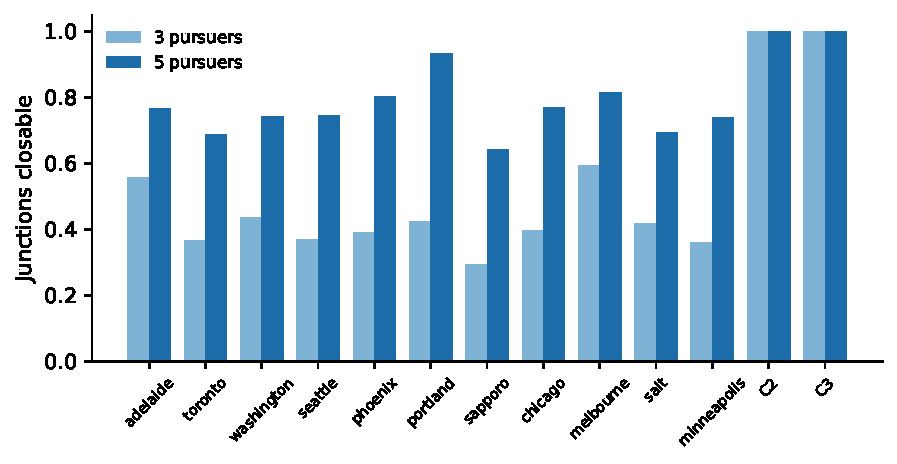
\includegraphics[width=\columnwidth]{F4_junction_blockability.pdf}
\caption{Share of junctions whose exit lanes can be closed by three or five pursuers, by network.}
\label{fig:blockability}
\end{figure}

\emph{Structure.} Closing a junction needs a median of 3--4 lanes on real downtowns. A team of three can close 30--59\%
of junctions, against 100\% on the grids (Fig.~\ref{fig:blockability}). On TEST, observed capture by PLB falls from
0.43 (at most 4 lanes to close at the evader's first junction) to 0.32 (5--6 lanes) and 0.12 (at least 7). This is an
association, not an identified causal ceiling. It agrees in kind with a cellular-automaton study of a three-lane
ring road, in which one learned interceptor slowed a target and two, blocking two lanes, stopped it
\cite{bykov2025interceptor}.

\emph{Prediction and speed.} An oracle that knows the evader's decision function predicts its next turn with 95--98\%
accuracy at short lead, against about 50\% for the greedy predictor. It changes capture by $+0.03$ to $+0.04$, with
intervals that include zero. Pursuers 1.1 or 1.2 times faster change capture by $-0.07$ to $+0.03$. Neither result
establishes equivalence; neither indicates a large gain.

\subsection{Learning: No Validated Gain over Imitation}
\label{sec:limit}

Fine-tuning the imitation controllers gave no validated gain, in three successive implementations. With the first
(MAPPO-v2), fine-tuning lowered validation capture in all four runs, from 0.36--0.37 to 0.20--0.22 within 2\,048
training attempts. An audit then found that its critic received a state that depended on the actions of the step. In
a repetition with a corrected controller (MAPPO-v3) and new scenarios, the decline did not recur. That repetition
changed the critic input, the sampling and the scenarios together, so it does not isolate the cause of the earlier
decline.

A further audit found two defects in the training loop that these studies shared. The last decision of an episode
was trained although it has no future inside the episode: at the 300\,s horizon whenever the objective was not
reached, and at the capture instant when it fell on a decision tick. And the collision penalty came from an
episode-level flag, so a collision after the cut would have penalized a finished prefix. Neither defect touches
behaviour cloning or the scoring of a stored policy. We corrected the loop, added a ledger with one row per training
episode, and repeated the registered study (MAPPO-v4) with the same arms, seeds, budgets, imitation starts and
training scenarios, and new test scenarios. Each run made 2\,048 training attempts. Of the 16\,384 attempts of
fine-tuning, 16\,026 were valid episodes; the critic warm-up, which was applied to the MLP head only, added 503
valid episodes of 512 attempts. In these 16\,529 episodes the earlier loop would have trained 6\,281 decisions
without a future (0.6\% of its decisions, in 38\% of the episodes); no collision occurred.

The outcome did not change. In the six runs rewarded with OC (the MLP head with and without a critic warm-up, and
the KAN head without), validation capture stayed between 86 and 92 of 190 valid validation episodes over the 2\,048
training attempts of a run, from starts of 88 to 90. No run reached the registered gain, the breakers kept the
imitation starts, and the registered primary, a validated improvement on imitation, was not met. On fresh scenarios
(22\,316 episodes) the final policies differ from their starts by $+0.011$ [$-$0.005, 0.026], $0.000$
[$-$0.012, 0.013] and $+0.010$ [$-$0.001, 0.021] in the three arms; in MAPPO-v3 these were $+0.015$, $+0.009$ and
$+0.003$. No consistent deterioration was observed, and no validated gain was obtained at this budget. The intervals
include small losses as well as small gains, and no test of equivalence or non-inferiority was made. Two seeds per
arm do not estimate the variability between training runs, the imitation policies are nearly deterministic, so
fine-tuning explored little, the learner was not tuned, and a difference between two implementations is not
attributed to a cause (supplement, Section~S-IV).

The imitation controllers themselves, which hold each decision for 3\,s, do not lag the planner that they copy: they
differ from PLB by $-0.009$ to $+0.047$ across six test sets, with an interval above zero in two of them, one
analysed post hoc. The cause of that small difference is not established: a registered test of the 3\,s commitment
was not confirmed (supplement, Section~S-IV). The negative result is therefore specific: for this controller and
these budgets, reinforcement learning did not improve on the imitation of PLB. It is not evidence that learned
controllers cannot match or exceed a planner.

\emph{Kolmogorov--Arnold models (exploratory, post hoc).} We fitted a KAN, a spline-additive logistic model, an MLP
and a logistic regression to predict capture from six start-state features, and compared them on matched estimands
with a bootstrap over true scenario families. On TEST, the AUC is 0.597 for the KAN, against 0.645 (spline-additive),
0.647 (MLP) and 0.646 (logistic). No KAN advantage was detected, in line with controlled comparisons of KANs and MLPs
\cite{yu2024kanfair}; this does not establish equality. Our earlier use of a KAN to interpret learned pursuit
policies \cite{noguera2025kan} did not include such a comparison. All four models describe the same association, a logit that
falls with the number of lanes to close, and we do not claim a KAN-specific interpretability advantage (supplement,
Section~S-V).

% =====================================================================================================
\section{Discussion and Reporting Checklist}
\label{sec:discussion}

\emph{What success means.} In real downtown traffic, proximity endpoints register success even when nobody pursues,
and they disagree with operational stopping by a factor of three to five. In the official environments of two
published methods, the capture rule was met only by vehicles crossing paths, and a team turning at random met it
several times as often as a team that chases. For simulation-based pursuit research this is a question of validity:
a success rate can be interpreted only together with what its capture rule rewards.

\emph{Getting ahead.} Under the audited endpoint, waiting in the predicted exit lanes outperforms chasing on two
held-out sets of cities and across evader behaviours. The size of the advantage is not stable: 14.5 points on one
set and 6.4 on the other, and PLB is distinguishable from the simpler junction ambush on the first only. This agrees
with prepositioning in fugitive interception \cite{vandroffelaar2024simopt}, now under microscopic constraints. A
same-budget ablation shows that joint assignment adds 7 points of capture, growing with team size, whereas the team
shows no statistically supported excess over an independence reference. The diagnostics are consistent with joint
assignment reducing interference, and capture is associated with the number of lanes to close; neither is established
as the mechanism or as a bound.

\emph{Learning.} For the controllers and budgets tested, fine-tuning produced no validated improvement on
imitation, in the original study and in two registered repetitions made after audits found defects in the training
code; the imitation controllers differ little from the planner they copy. An earlier report that fine-tuning
degraded them did not recur. Some of the defects were found after results had been reported: negative results about
learning need the same audit as positive ones. We do not conclude that learning cannot help: richer action spaces,
more exploration, longer training or adversarial evaders may change this.

\emph{A reporting checklist.} The audits suggest six items that a pursuit study can report at low cost. They ask for
reporting, not for the adoption of our endpoint, which is itself fallible:
\begin{enumerate}
\item \textbf{The capture rule in full:} which points of the vehicles the distance joins, the speeds allowed, and
whether the evader is removed at capture.
\item \textbf{Null-team calibration:} the score of a team that does not pursue, under the same rule.
\item \textbf{A hold audit:} what the evader does in a fixed time after capture, with complete follow-up.
\item \textbf{Containment indicators:} for any such indicator, the share of certified evaders that escape, counting
exits from the network.
\item \textbf{Held-out evaluation:} an evaluation on networks not used for design, opened once, with intervals
clustered by scenario.
\item \textbf{Registration:} which analyses were registered before the runs and which were not.
\end{enumerate}

% =====================================================================================================
\section{Limitations and Threats to Validity}
\label{sec:limitations}

We group the threats by the kind of validity they affect, and state what was done about each.

\emph{What OC measures.} OC is an operational near-stop endpoint. It admits slow following behind a pursuer (null-team
floor about 3\%), requires no rear blocker, and its 0.3--2\,m band is tied to the evader's 1.0\,m minimum gap.
Persistence was tested against scripted evaders and SUMO's lane changing; an active lane-change probe released 15 of
1\,433 captures. Reversing and mid-edge U-turns were not evaluated, which favours blocking.

\emph{The simulator.} Every result comes from one microscopic simulator. SUMO moves vehicles along lanes with a
longitudinal car-following law and discrete lane changes. It has no tyre or steering dynamics, and its drivers do not
ram, mount kerbs or drive against traffic. Two checks probe this limit from inside the simulator (supplement,
Section~S-VI). First, on fresh scenarios we changed the position-update rule (ballistic instead of Euler) and the
car-following model (IDM instead of Krau{\ss}). PLB minus pursuit is $+0.126$ [0.090, 0.164] with the model used
throughout, $+0.140$ [0.103, 0.177] with the ballistic update and $+0.118$ [0.079, 0.158] with IDM, and the 5\,m rule
exceeds OC for the pursuit team by 0.58--0.63 in all three. Second, we added background traffic, about 300 random-trip
cars per city, which until then had been tested only for pursuit. PLB minus pursuit is then $+0.094$ [0.060, 0.130].
Traffic lowers capture by PLB by 6 points and by pursuit by 3. The advantage observed with traffic is 3 points
smaller than without, but the interval of that difference reaches zero ([$-$0.066, 0.000]), so a smaller advantage on
busy streets is not established. These checks do not replace a different simulator or field data.

\emph{The evaders.} All evaders are scripted and decide from the pursuers' current positions. The evader tuned
against PLB (Section~\ref{sec:evaders}) is a rule with seven hand-chosen features and 33 candidates, tuned by random
search; a stronger evader may exist. Learned evaders exist in SUMO pursuit \cite{wang2022opponent} and were not
evaluated, and no game-theoretic best response was computed.

\emph{Inference.} There are eight held-out cities, in two sets that were each evaluated once and are not pooled;
the advantage of PLB differs between the sets, and we did not identify why. DEVELOPMENT cities informed design.
Registration is internal. The independence reference is not a causal test of cooperation; the coordination ablation
is, but only for joint assignment within PLB. The published-environment audits used the released configurations,
which differ from the reported ones, did not train the published learners, and cover two environments of one
research group.

\emph{Reproducibility.} Packages store source hashes rather than complete source snapshots, so the launch versions of
some earlier studies cannot be recovered in full. Replays reproduced every sealed outcome that we re-ran, and a
correction to the bookkeeping of rejected commands changed no outcome in 8\,966 re-runs (supplement,
Section~S-VII).

% =====================================================================================================
\section{Conclusion}
\label{sec:conclusion}

In microscopic urban traffic, proximity and operational interception answer different questions. A 5\,m rule scores
three to five times more successes than an operational stop on held-out downtowns, scores about a third of episodes
as successful when nobody pursues, and hides or reverses the advantage of one controller over another. In the
official environments of two published methods, the capture rule was met only by vehicles crossing paths, and a team
turning at random met it far more often than a team that chases. The operational endpoint we use persisted in every
audited case when the pursuers held under the scripted evaders. An active lane-changing probe produced 15 escapes, so
the endpoint does not guarantee containment. A lane-level containment indicator is useful but fallible, while a
junction-level indicator is not reliable.

Under this audited measurement, predictive lane blocking is a strong baseline. It beats pursuit by 14.5 points on one
held-out set of four cities and by 6.4 points on a second, and by 9 to 21 points on the development cities against
five evader behaviours, one tuned against it, under two alternative kinematic models and with background traffic.
Joint assignment matters: removing it costs 7 points. Fine-tuning a learned controller gave no validated gain over
imitation for the budgets tested, also after its training code had been corrected twice. All of this is simulation
with scripted evaders; the checklist of Section~\ref{sec:discussion} states what we believe a pursuit study should
report so that its success rates can be interpreted.

% =====================================================================================================
\section*{CRediT authorship contribution statement}
\textbf{Andrei Noguera Gil:} Conceptualization, Methodology, Software, Validation, Formal analysis, Investigation,
Data curation, Writing -- original draft, Visualization, Project administration.
\textbf{Felix Martinez-Rios:} Conceptualization, Methodology, Supervision, Writing -- review \& editing.
\textbf{Edgar Avalos-Gauna:} Conceptualization, Validation, Writing -- review \& editing.

\section*{Declaration of competing interest}
The authors declare that they have no known competing financial interests or personal relationships that could have
appeared to influence the work reported in this paper.

\section*{Funding}
This research did not receive any specific grant from funding agencies in the public, commercial, or not-for-profit
sectors.

\section*{Data availability}
The code, the sealed evidence packages with SHA-256 checksums, the pre-registration records, the versioned audit
addenda and the analysis scripts are archived at Zenodo \cite{noguera2026code} and developed at
\url{https://github.com/Andnog/pursuit-capture-audit}, which also gives the instructions to verify them and to run
every study again. The run logs and pickled training states of the packages (552\,MB), which the repository lists
with their sealed checksums, are deposited separately. \pending{add the DOI of the second Zenodo deposit, the heavy
files, and cite it as a dataset}

\section*{Declaration of generative AI and AI-assisted technologies in the manuscript preparation process}
During the preparation of this work the authors used Claude Opus~5.5 (Anthropic) in order to draft and edit text of
the article and its supplement, to organize the literature and to collate and format the reference list, and to draw
the schematic of Fig.~\ref{fig:method}; and Astra, through the ChatGPT desktop application (OpenAI), in order to
check the code, the results and the manuscript for errors, for internal consistency and against the journal's
guidelines. Both were used under the supervision of the first author. Every reference was verified by the authors
against its source. After using these tools, the
authors reviewed and edited the content as needed and take full responsibility for the content of the published
article. The use of AI tools in the research process (code, experiments, analysis, data figures and audits) is
described in Section~\ref{sec:protocol}.

\bibliographystyle{elsarticle-num}
\bibliography{refs}

\end{document}
